% \documentclass[handout]{beamer}
\documentclass{beamer}

% \usetheme{boxes} % see http://www.deic.uab.es/~iblanes/beamer_gallery/ for lots of examples
\usetheme{metropolis}
\usecolortheme{rose}
% \useinnertheme{circles}
% \useoutertheme{split}
% \setbeamertemplate{blocks}[rounded][shadow=true]

\setbeamertemplate{navigation symbols}{} % remove navigation symbols
\setbeamertemplate{footline}{} % remove title, too long

% %next set colors - not needed
% \setbeamercolor{title}{fg=black!70!black}
% \setbeamercolor{frametitle}{fg=blue!70!black}
% \setbeamercolor{framesubtitle}{fg=green!30!black}
% \setbeamercolor{author}{fg=red!70!black}
% \setbeamercolor{institute}{fg=green!30!black}
% \setbeamercolor{date}{fg=blue!50!black}

% \usepackage[T1]{fontenc}        % kodiranje znakov v .pdf
% \usepackage[utf8]{inputenc}     % kodiranje znakov v .tex
% \usepackage[slovene]{babel}     % nastavimo slovenščino
% \usepackage{stmaryrd}

\usepackage{fontspec}
\usepackage{mathtools}
\usepackage{unicode-math}
\usepackage{enumerate}

\usepackage{graphicx}
\usepackage{tabulary}


\setmainfont{Latin Modern Roman}
% \setmainfont{TeX Gyre Pagella}
% \setmathfont{TeX Gyre Pagella Math}
\setmathfont{Latin Modern Math}
\setmathfont{Asana Math}[range={scr}]
\setmathfont{STIX Two Math-Regular}[range={bb,"1D538-"1D56B,"0211D}]
\setmathfont{STIX Two Math-Regular}[range={"2102,"210D,"2115,"2119,"211A,"211D,"2124}]
% \setmathfont{TeX Gyre Pagella Math}[range={8730}] %sqrt
% \setmathfont{Asana Math}[range={"007B,"007D}]  % {}
\setmathfont{Asana Math}[range={8709,\setminus,"2216,"29F5,"219D}]  % U+2205, emptyset
\setmathfont{Asana Math}[range={10631, 10632}]  % U+2987, U+2988, bb parenthesis

\usepackage[normalem]{ulem}
\renewcommand{\ULdepth}{1.8pt}
\newcommand{\ul}[1]{\uline{#1}}


\usepackage{amsfonts,amsmath,amssymb,amsthm}
\theoremstyle{theorem}
\newtheorem{izrek}{Theorem}
\newtheorem{trditev}{Proposition}
\newtheorem{lema}{Lemma}
\newtheorem*{posledica}{Corollary}

\theoremstyle{definition}
\newtheorem{definicija}{Definition}

\newtheorem*{primer}{Example}
\newtheorem*{primer*}{Example}
\newtheorem*{primeri}{Examples}

\theoremstyle{remark}
\newtheorem*{opomba}{Remark}

% \beamertemplatetransparentcovereddynamic

\makeatletter
\let\authorfield\author
\let\institutefield\institute
\renewcommand{\author}[1]{\def\@author{#1}}
\renewcommand{\institute}[1]{\def\@institute{#1}}
\newcommand{\location}[1]{\def\@location{#1}}
\title{Topological Properties are Logical Principles in Topological Models}
% \author{Luna Strah\\ {\scriptsize University of Ljubljana, Faculty of mathematics and physics}}
\author{Luna Strah}
\institute{University of Ljubljana, Faculty of mathematics and physics}
\location{Syntax and Semantics of Type Theory 2026}
% \institute{University of Ljubljana, Faculty of mathematics and physics}
%\institute{Syntax and Semantics of Type Theory 2026}
\date{4.~6.~2026, Ljubljana}
\authorfield{\@author\\ {\scriptsize \@institute}}
\institutefield{\@location}
\makeatother

\newcommand{\eps}{\varepsilon}
\renewcommand{\hat}{\widehat}
\renewcommand{\tilde}{\widetilde}
\renewcommand{\bar}{\overline}


\def\bN{\mb{N}}
\def\bR{\mb{R}}
\def\subq{\subseteq}
\def\phi{\varphi}

\DeclarePairedDelimiterX{\parens}[1]{(}{)}{#1}
\DeclarePairedDelimiterX{\absolute}[1]{\lvert}{\rvert}{#1}
\def\abs{\absolute*}
\newcommand{\cli}[1]{\left[ {#1} \right]}
\newcommand{\floor}[1]{\left\lfloor {#1} \right\rfloor}
\newcommand{\set}[2]{\left\{ #1 \mid #2 \right\}}
\newcommand{\apart}{\ensuremath{\mathrel{\#}}}
\newcommand{\nbd}{\oset{\text{\clap{\tiny nbd}}}{∋}}
\newcommand{\quot}[2]{{#1}/_{\!#2}}
\newcommand{\mb}[1]{\mathbf{#1}}
\newcommand{\bb}[1]{\mathbb{#1}}
\newcommand{\mf}[1]{\mathfrak{#1}}
\newcommand{\mc}[1]{\mathcal{#1}}
\newcommand{\cat}[1]{\mathbf{#1}}
\newcommand{\opcat}[1]{\left(\mathbf{#1}\right)^{op}}
%\newcommand{\op}[1]{{#1}^{op}}
\newcommand{\op}{\oset{\text{op}}{⊆}}
\newcommand{\res}[1]{\hspace{-0.2em}↾_{\hspace{-0.15em}#1}}
% \newcommand{\res}[2]{#1{↾_{\hspace{-0.15em}#2}}}
\newcommand{\sh}[1]{\textrm{Sh}{\left( #1 \right)}}
%\newcommand{\psh}[1]{\textrm{PSh}{\left( #1 \right)}}
\newcommand{\psh}[1]{\hat{#1}}
\DeclareMathOperator{\im}{im}
\DeclareMathOperator{\coker}{coker}
\DeclareMathOperator{\coim}{coim}
\DeclareMathOperator{\id}{id}
\DeclareMathOperator{\codim}{codim}
\DeclareMathOperator{\cl}{cl}
\DeclareMathOperator{\ext}{ext}
\DeclareMathOperator{\dom}{dom}
\DeclareMathOperator{\ev}{ev}
\DeclareMathOperator{\el}{el}
\DeclareMathOperator{\dm}{DM}
%\DeclareMathOperator{\cov}{Cov}
\AtBeginDocument{
  %\def\c#1{\left( {#1} \right)^c}
  %\def\c#1{{#1}^c}
  \def\c{\uline}
  \def\h{ℋ}
  \def\hvsets{\cat{HVSets}}
  \newcommand{\g}[1]{\left\langle {#1} \right\rangle}
  \renewcommand{\b}[1]{\left\{ {#1} \right\}}
  \renewcommand{\i}[1]{\left⟦ {#1} \right⟧}
  % \newcommand{\e}[1]{\left‖ {#1} \right‖}
  \newcommand{\eq}[3][]{{#2} \sim_{#1} {#3}}
  \DeclareMathOperator{\e}{E}
  \newcommand{\carr}[1]{\left\vert {#1} \right\vert}
  \newcommand{\s}[1]{\left\{ {#1} \right\}}
  \renewcommand{\O}[1]{\mathcal{O}{#1}}
  \renewcommand{\int}{\textrm{int}}
  \def\p{\parens*}
}


\newcommand{\defquantifier}[2]{%
  \expandafter\undef\csname #1\endcsname%
  \expandafter\newcommand\csname #1\endcsname[2]{{#2 ##1.}\;##2}%
}
\defquantifier{for}{\forall}
\defquantifier{exist}{\exists}
\defquantifier{unique}{\exists!}
%\defquantifier{globalen}{\exists ᵍ}
\defquantifier{exact}{ι}
\defquantifier{eventually}{\nabla}
\AtBeginDocument{
\renewcommand{\sigma}[2]{(#1)×#2}
%\defquantifier{sigma}{\Sigma}
\defquantifier{pi}{\Pi}
}
\renewcommand{\check}{ \(\checkmark\)}

\newcommand{\germ}[2]{\textrm{germ}_{#2}#1}
%\usepackage{xparse}
\makeatletter
\NewDocumentCommand{\@defprinciple}{mmm}{%
  \ExpandArgs{c}\NewDocumentCommand{#1}{s}{%
    \IfBooleanTF##1%
    {\textnormal{\sffamily #2}}%
    {\textnormal{\sffamily #3}}%
  }%
  \AtEndPreamble{%
    \pdfstringdefDisableCommands{%
      \expandafter\def\csname #1\endcsname*{#2}%
    }%
  }%
}
\newcommand{\defprinciple}[1]{\@defprinciple{#1}{\MakeUppercase{#1}}{\MakeLowercase{#1}}}
\makeatother
\newcommand{\principle}[1]{\textnormal{\sffamily #1}} % TODO: rename
\defprinciple{lem}
\defprinciple{wlem}
\defprinciple{lpo}
\defprinciple{wlpo}
\AtBeginDocument{
\undef\mp
\defprinciple{mp}
}
\defprinciple{ks}
\defprinciple{alpo}
\defprinciple{awlpo}
\defprinciple{allpo}
\defprinciple{amp}
\defprinciple{awmp}
\defprinciple{aks}
\newcommand{\AC}{\principle{AC}}
\newcommand{\IAC}{\principle{IAC}}
\newcommand{\CC}{\principle{CC}}
\newcommand{\MetaCC}{\principle{MetaCC}}
\newcommand{\CCv}{\principle{CC}^∨}
\newcommand{\DC}{\principle{DC}}
\def\Rm{ℝ_{\text{M}}}
\def\Rd{ℝ_{\text{D}}}
\def\Rc{ℝ_{\text{C}}}
\def\Ncof{ℕ^{\text{cof}}}

\setbeameroption{hide notes} % Only slides
% \setbeameroption{show only notes} % Only notes
% \setbeameroption{show notes} % Both
% \setbeameroption{show notes on second screen=right} % Both

\usepackage{hyperref}
\hypersetup{pdfpagemode=FullScreen}

\usepackage[style=alphabetic,
            hyperref=auto,
            isbn=false,
            doi=true,
            url=false,
            date=year,
            giveninits=true,
            maxnames=3,
            useprefix=true,
            backend=biber]{biblatex}
\bibliography{../src/magisterij.bib}

\begin{document}
%%%%%
\frame{
  \titlepage

  \note{
  }
}
\frame{
  Formulas can be assigned open sets, thus logical principles (that therefore
  talk about open sets) can be interpreted as topological properties.

  \note{
  }
}
% \begin{frame}
%   \frametitle{Blackboard content}
%   \begin{figure}
%     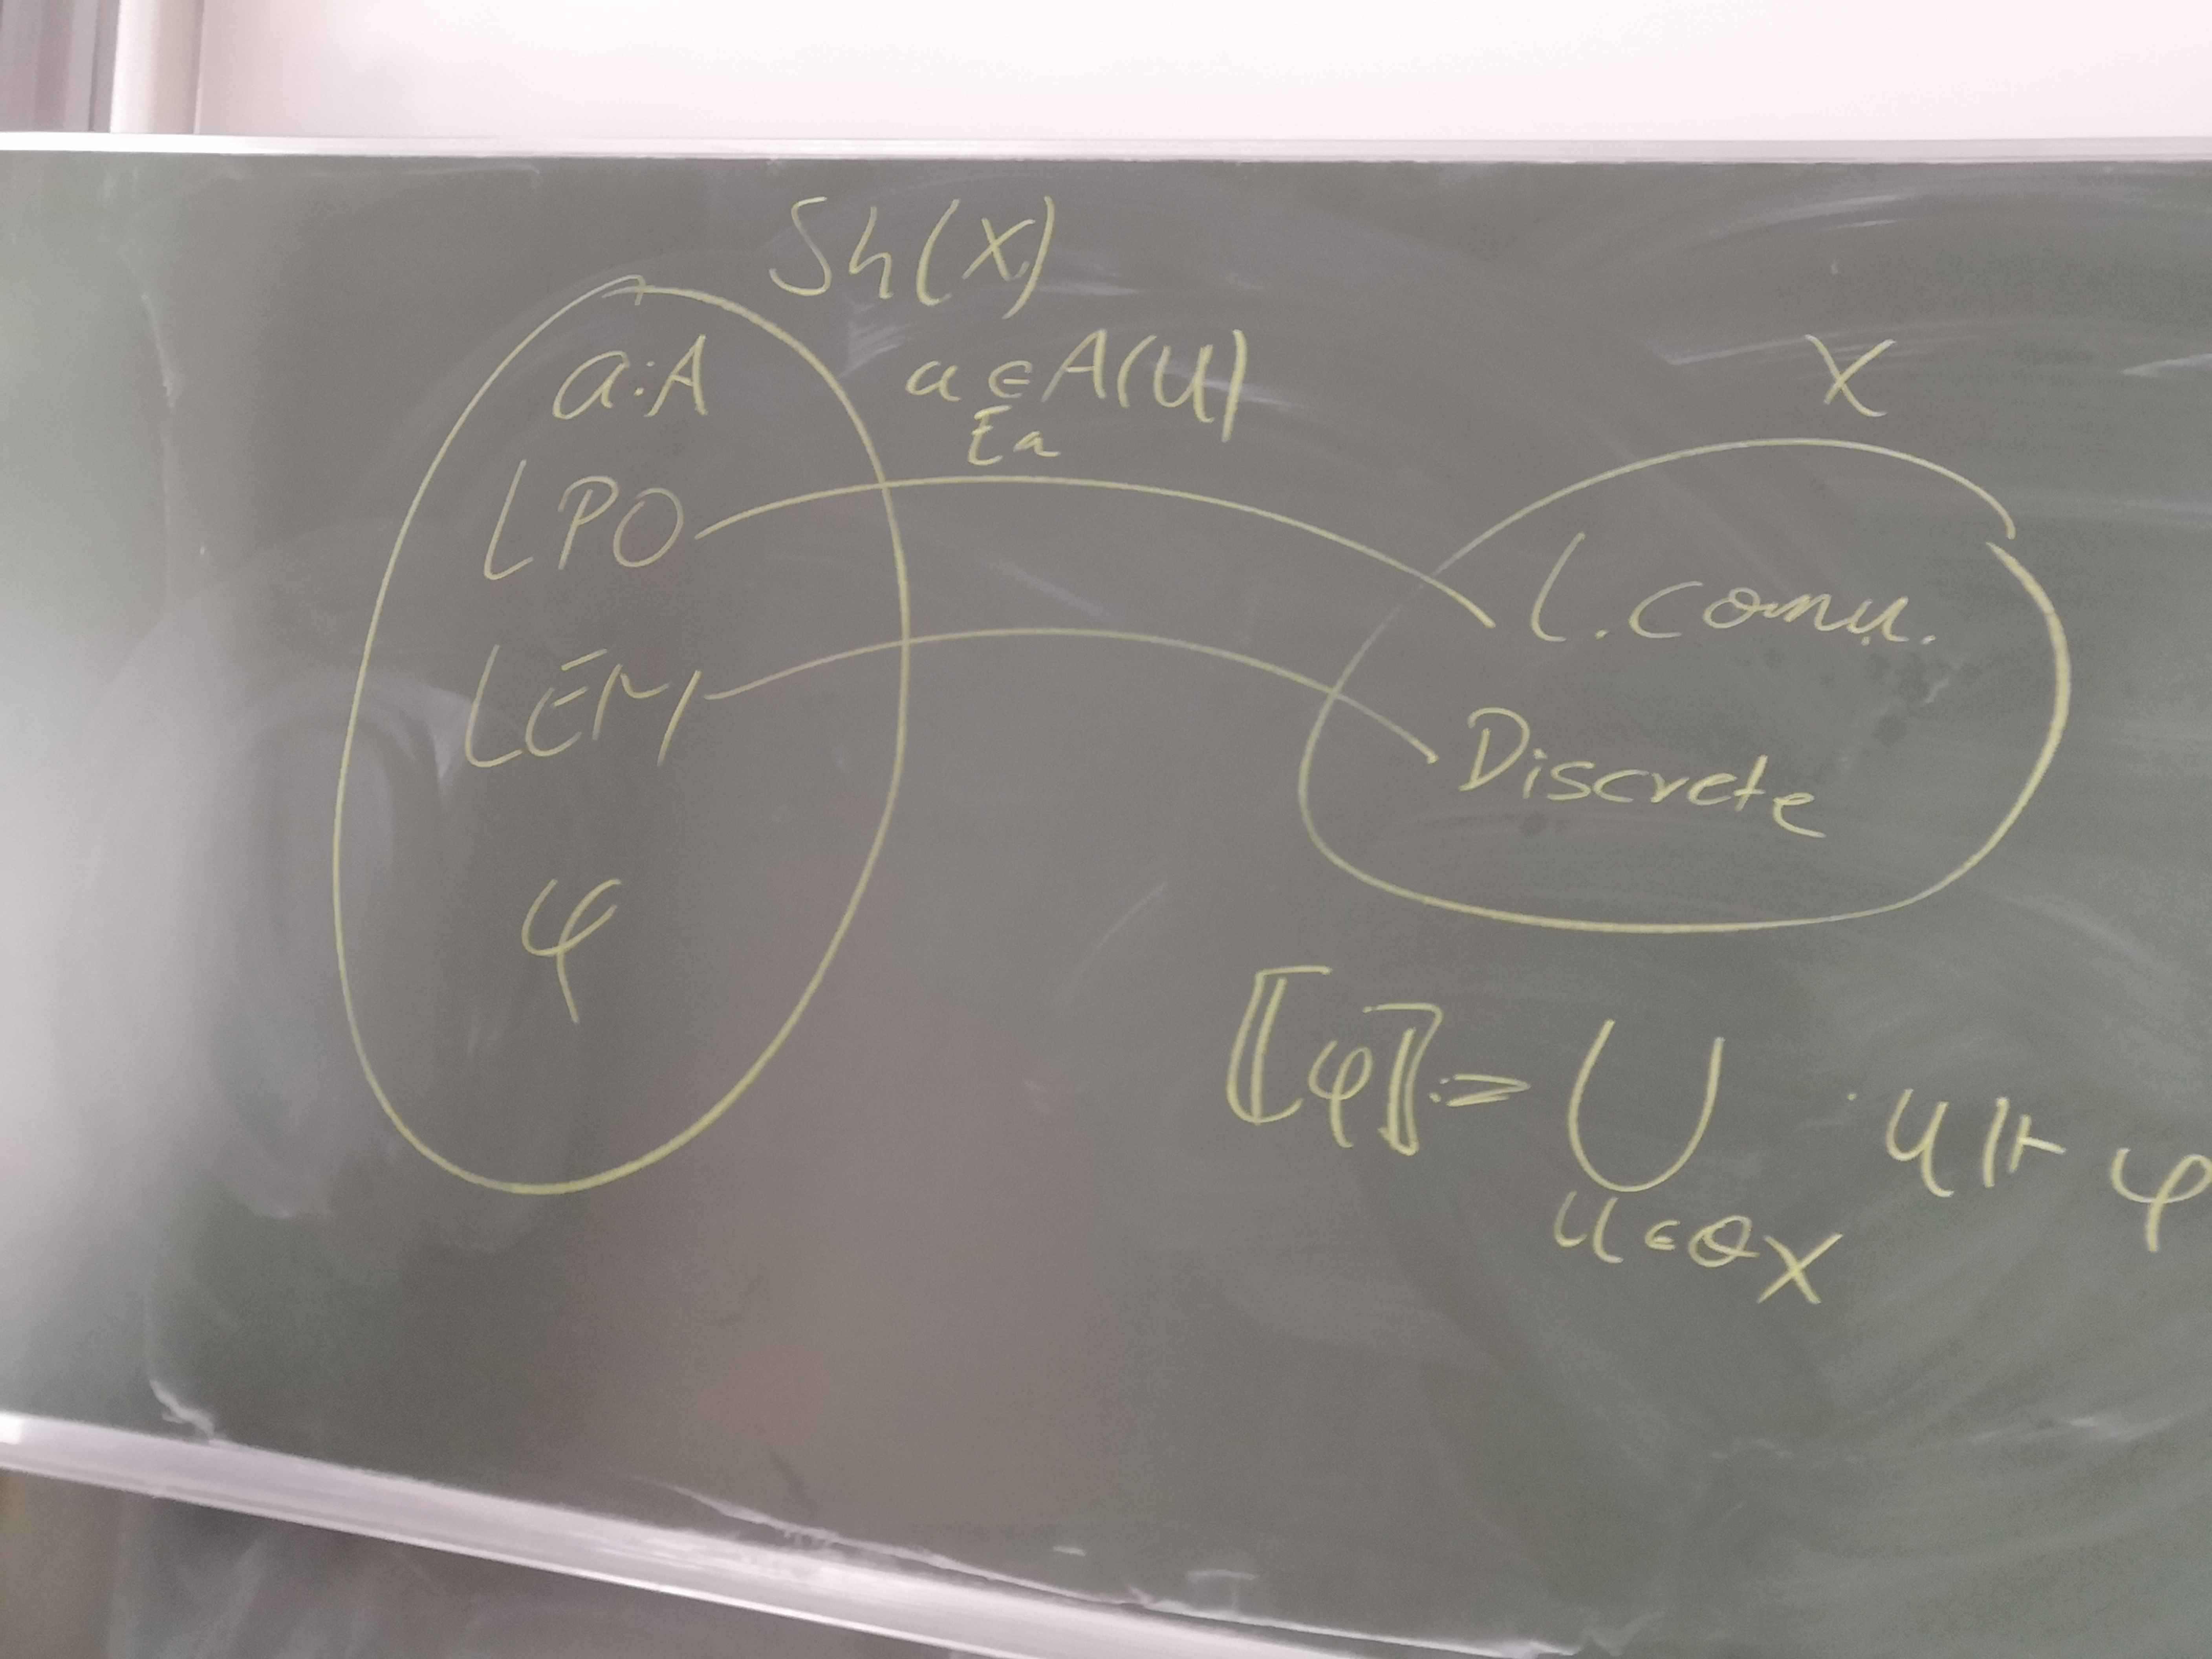
\includegraphics[width=0.9\textwidth]{board-1.jpg}
%   \end{figure}
% \end{frame}

%%%%%
% TODO: Slides about synteticness and what we are doing

% \begin{frame}
%   \frametitle{Logic of Open Sets}

%   \begin{align*}
%     &\i ⊤                    ≔ X\\
%     &\i ⊥                    ≔ ∅\\
%     &\i{φ ∧ ψ}               ≔ \i φ ∩ \i ψ\\
%     &\i{φ ∨ ψ}               ≔ \i φ ∪ \i ψ\\
%     &\i{φ ⇒ ψ}               ≔ \int{\p{\i ψ ∪ \i φᶜ}}\\
%     &\i{\for{x : A}{φ(x)}}   ≔ \int{⋂_{a ∈ A}\i{\e a ⇒ φ(a)}}\\
%     &\i{\exist{x : A}{φ(x)}} ≔ ⋃_{a ∈ A}\i{\e a ∧ φ(a)}
%     % &\i{τ = σ}               ≔ ⋁\set{V}{τ\res V = σ\res V}\\
%     % &\i{R(τ)}                ≔ R{\p{\i τ_A}}\text{, for a relation \(R\) on \(A\) and \(τ : A\)}
%   \end{align*}
%   \note{
%     Formula \(φ\) je veljavna na \(U\), ko je \(U ⊆ \i φ\).
%   }
% \end{frame}

% \begin{frame}
%   \frametitle{Objects}

%   \(A\) set, \(T\) topological space
%   \[ T_X(U) ≔ 𝒞(U, T) \]
%   For \(X = ℝ\) the map \(\id : ℝ → ℝ\) is a Dedekind real number.

%   The constant type \(\c A\) is the sheaf \(\c A (U) ≔ A\).

%   \note{
%     \(\Rc, \Rd, \Rm, \c ℝ, Ω\), Cantor
%   }
% \end{frame}

% \begin{frame}
%   \frametitle{Blackboard content}
%   \begin{figure}
%     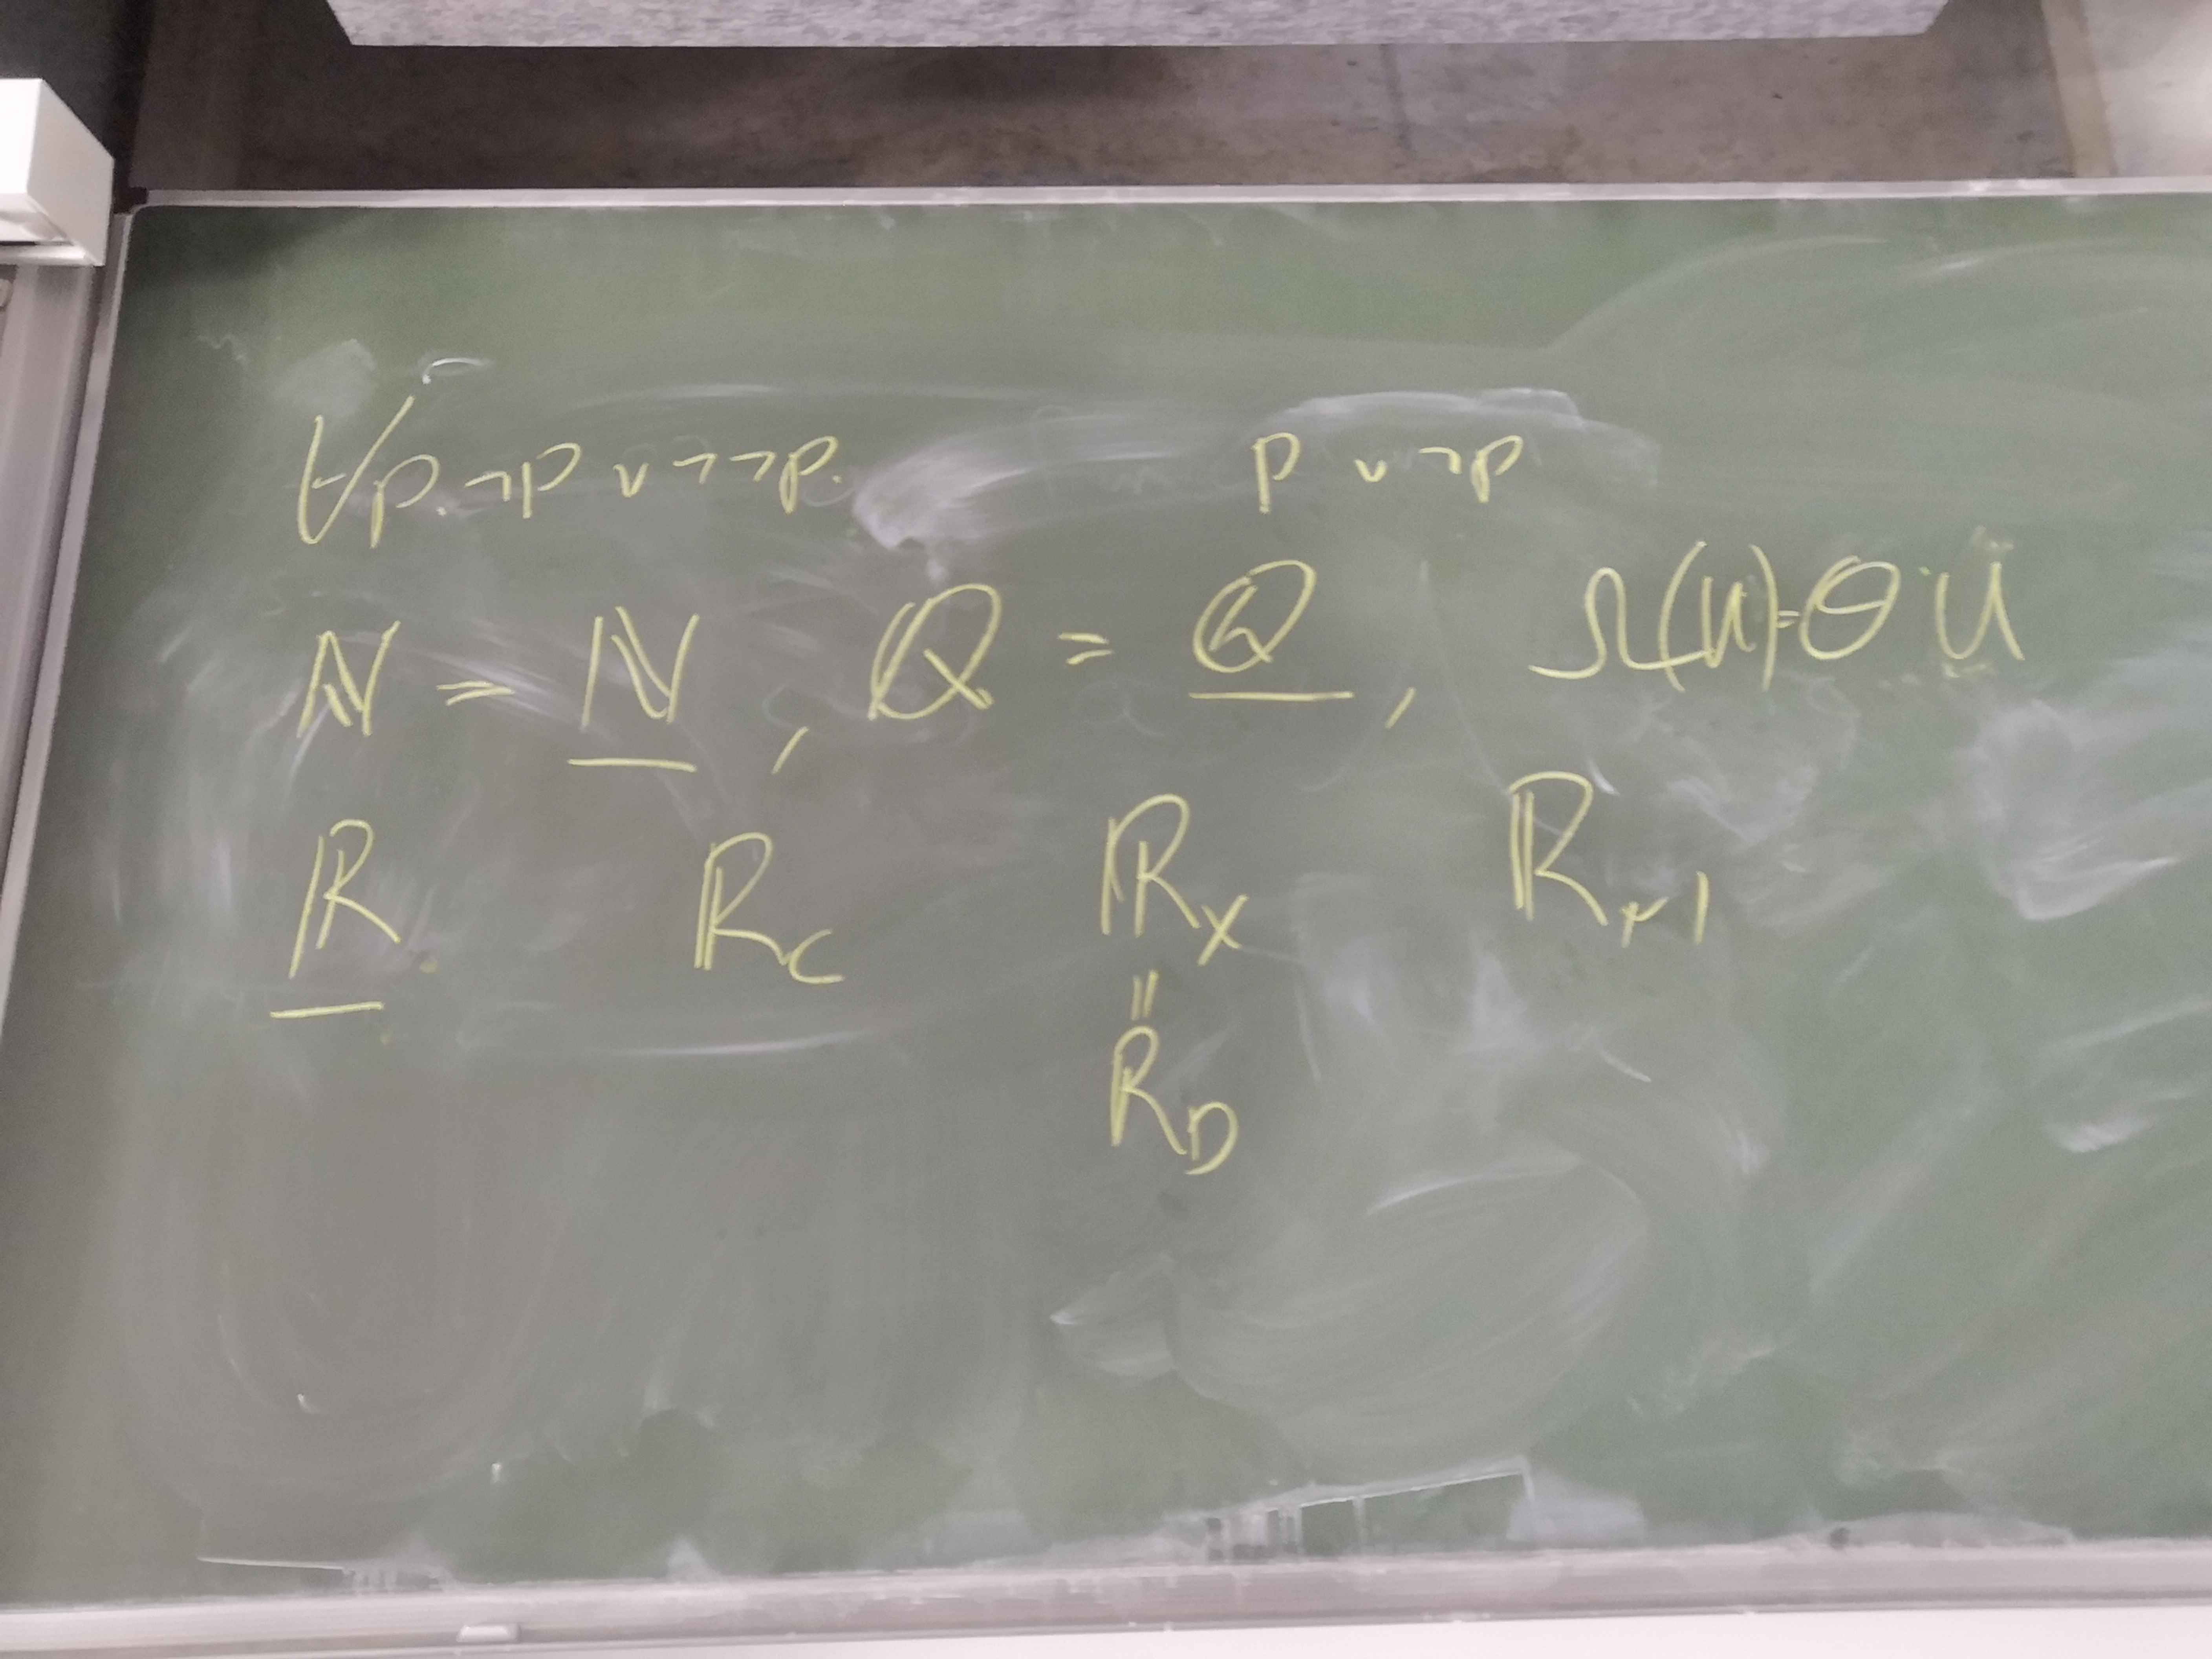
\includegraphics[width=0.9\textwidth]{board-2.jpg}
%   \end{figure}
% \end{frame}

\begin{frame}
  \frametitle{\(\lem*\) and company}

  \begin{trditev}
    A space is discrete iff it satisfies \(\lem*\).

    A space is extremally disconnected iff it satisfies \(\wlem*\) (\(\for{p:Ω}{¬p ∨ ¬¬p}\)).
  \end{trditev}
\end{frame}

\begin{frame}
  \frametitle{What about theorems?}

  An extension to the observation then, is that theorems in constructive logic become theorems of topological properties.

  \begin{trditev}
    \(\lem* ⇒ \wlem*\)
  \end{trditev}

  \begin{corollary}
    Every discrete space is extremally disconnected.
  \end{corollary}
\end{frame}

\begin{frame}
  \frametitle{Sample theorems}

  \begin{trditev}
    \[ \lpo* ⇔ \wlpo* ∧ \mp* \]
  \end{trditev}
  \begin{trditev}
    \[ \wlem* ⇔  \Rd ≡ \Rm\]
  \end{trditev}
\end{frame}

\begin{frame}
  \frametitle{Principles}

  \begin{align*}
    &\lpo* ≔ \for{α : 2^ℕ}{α = 0 ∨ α \apart 0}\\
    &\wlpo* ≔ \for{α : 2^ℕ}{α = 0 ∨ α ≠ 0}\\
    &\mp* ≔ \for{α : 2^ℕ}{α ≠ 0 ⇒ α \apart 0}\\
    &\alpo* ≔ \for{x : \Rd}{x = 0 ∨ x \apart 0}\\
    &\awlpo* ≔ \for{x : \Rd}{x = 0 ∨ x ≠ 0}\\
    % \pause
    &\amp* ≔ \for{x : \Rd}{x ≠ 0 ⇒ x \apart 0}
    % &\ks* ≔ \for{p : Ω}{\exist{α : 2^ℕ}{p ⇔ α \apart 0}}\\
    % &\aks*_ℛ ≔ \for{p : Ω}{\exist{x : ℛ}{p ⇔ x \apart 0}}
  \end{align*}

\end{frame}

% \begin{frame}
%   \frametitle{Choice}

%   Fix a subsheaf \(Σ ⊆ Ω\).

%   \begin{definicija}
%     Principle \(\AC_Σ(A,B)\) says, that every entire \(Σ\)-valued relation
%     \(R : A×B→Σ\) has a choice function.

%     \begin{align*}
%       &\AC_Σ(A) ≔ \for{B}{\AC_Σ(A,B)}\\
%       &\AC_Σ ≔ \for{A}{\AC_Σ(A)}\\
%       &\CC_Σ ≔ \for{B}{\AC_Σ(ℕ,B)}\\
%       &\CCv_Σ ≔ \AC_Σ(ℕ,2)
%     \end{align*}
%   \end{definicija}

% \end{frame}

% \begin{frame}
%   \frametitle{Choice}

%   \begin{definicija}
%     Principle \(\AC(A,B)\) says, that every entire relation \(R : A×B→Ω\) has a
%     choice function.

%     \begin{align*}
%       &\AC(A) ≔ \for{B}{\AC(A,B)}\\
%       &\AC ≔ \for{A}{\AC(A)}\\
%       &\CC ≔ \for{B}{\AC(ℕ,B)}\\
%       &\CCv ≔ \AC(ℕ,2)
%     \end{align*}
%   \end{definicija}

% \end{frame}

% \begin{frame}
%   \frametitle{Choice}

%   \begin{izrek}[Constructive]
%     Over \(X\) we have \(X ⊩ A^{ℕ} ≅ \c {\p{ΓA}^ℕ}\) for all \(A\) iff every
%     coutable family of covers has a joint refinement.
%   \end{izrek}

%   \begin{izrek}[Constructive]
%     For a space \(X\) satisfying either of the above we have
%     \[ X ⊩ \CC \text{ iff } \MetaCC\text. \]
%   \end{izrek}

%   \pause

%   \begin{izrek}[\cite{Simpson24}]
%     A Grothendieck topos satisfies \(\CC\) and
%     \[ \pi{n:ℕ}{\sigma{x:X}{A_{n,x}}} ≅ \sigma{f:ℕ → X}{\pi{n:ℕ}{A_{n,f(n)}}} \]
%     iff
%     it's Grothendieck topology is closed under countable intersections.
%   \end{izrek}
% \end{frame}

% \begin{frame}
%   \frametitle{Choice}

%   \begin{definicija}
%     A space is a \emph{P-space} when a countable intersection of opens is open.
%   \end{definicija}
%   \begin{trditev}
%     For a P-space every countable family of covers has a common refinement.
%   \end{trditev}
%   \begin{posledica}
%     P-spaces satisfy \(\CC\).
%   \end{posledica}

% \end{frame}

% \begin{frame}
%   \frametitle{Choice}

%   \begin{trditev}
%     Over \(\cli{0,1}\) with topology \(\set{[0,a)}{a ∈ \cli{0,1}} ∪ \{\cli{0,1}\}\)
%     every family of covers has a common refinement but is not a P-space.
%   \end{trditev}

%   \pause

%   \begin{trditev}
%     If every countable family of covers in a \(T₁\) space has a common
%     refinement it is a P-space.
%   \end{trditev}

%   \begin{trditev}
%     Over locally connected \(T₁\) spaces \(\CC\) is equivalent to \(\CCv\).
%   \end{trditev}

% \end{frame}

% \begin{frame}
%   \frametitle{Choice}

%   \begin{trditev}
%     A space is Alexandrov iff it satisfies \(\AC(\c A)\) for all sets \(A\).
%   \end{trditev}

%   \pause

%   \begin{trditev}
%     A space is discrete iff it satisfies \(\AC\).
%   \end{trditev}

%   \begin{izrek}
%     In topological models \(\AC\) is \emph{equivalent} to \(\lem*\).
%   \end{izrek}

% \end{frame}

\begin{frame}
  \frametitle{Dedekind construction}

  \begin{definicija}[Dedekind construction]\label{def:Rd}
    A pair \(\p{L, U} ∈ 𝒫(ℚ)²\) is a \emph{Dedekind cut} when
    \begin{enumerate}
    \item \(L\) is inhabited, lower, and upwards open
    \item \(U\) is inhabited, upper, and downwards open
    \item \(p ∈ L ∧ q ∈ U ⇒ p < q\) for any \(p\), \(q : ℚ\)
    \item \(p < q ⇒ p ∈ L ∨ q ∈ U\) for any \(p\), \(q : ℚ\)
    \end{enumerate}
  \end{definicija}

\end{frame}

\begin{frame}
  \frametitle{MacNeille construction}

  \begin{definicija}[MacNeille construction]\label{def:Rm}
    A pair \(\p{L, U} ∈ 𝒫(ℚ)²\) is a \emph{Dedekind-MacNeille cut} when
    \begin{enumerate}[a.]
    \item[1.] \(L\) is inhabited, lower, and upwards open
    \item[2.] \(U\) is inhabited, upper, and downwards open
    \item \(p ∈ L ⇔ \exist{q>p}{q ∉ U}\)
    \item \(q ∈ U ⇔ \exist{p<q}{p ∉ L}\)
    \end{enumerate}
  \end{definicija}

\end{frame}

% \begin{frame}
%   \frametitle{MacNeille construction}

%   \begin{trditev}[\cite{Johnstone02}]\label{th:Rm-maps}
%     The type of MacNeille reals is the sheaf
%     \[ \Rm(U) ≔ \set{\p{\uline f, \bar f}}
%       {\uline f : \uline 𝒞(U, ℝ), \bar f : \bar 𝒞(U, ℝ), \textsf{tight}}
%     \]
%     where \textsf{tight} is
%     \[
%       \uline f(t) = \liminf_{y → t}\bar   f(y)\qquad\text{ and}\qquad
%       \bar   f(t) = \limsup_{y → t}\uline f(y)\text.
%     \]
%   \end{trditev}

% \end{frame}

% \begin{frame}
%   \frametitle{Reals}

%   For \(ℛ = \c ℝ\) the analytic principles are true.

%   For \(ℛ = \Rc\) the analytic and ``semi-decidable'' principles coincide.

%   \pause

%   For \(ℛ = \Rm\) the analytic principles correspond to full principles, so
%   \(\alpo*_{\Rm} = \amp*_{\Rm} = \lem*\) and \(\awlpo*_{\Rm} = \wlem*\).

%   Fix \(ℛ ≔ \Rd\).

% \end{frame}

\begin{frame}
  \frametitle{Reals}

  \begin{definicija}
    A space is a \emph{P-space} when zero sets of real-valued continuous functions \(U → ℝ\) are open.
  \end{definicija}
  \begin{trditev}
    A space satisfies \(\alpo*\) iff it is a P-space.
  \end{trditev}
  % \begin{trditev}
  %   A completely regular space satisfies \(\alpo*\) iff it is a P-space.
  % \end{trditev}

  \note{
    But remember P-space gives \(\CC\).
  }
\end{frame}

\begin{frame}
  \frametitle{Reals}

  \begin{definicija}
    A space is \emph{basically disconnected} when the closure of every cozero set is open.
  \end{definicija}
  \begin{trditev}
    A space satisfies \(\awlpo*\) iff every open subspace is basically
    disconnected.
  \end{trditev}

\end{frame}

\begin{frame}
  \frametitle{Reals}

  \begin{definicija}
    A space is an \emph{almost P-space} when every cozero set is regular.
  \end{definicija}
  \begin{trditev}
    A space satisfies \(\amp*\) iff every open subspace is an almost P-space.
  \end{trditev}

\end{frame}

\begin{frame}
  \frametitle{Reals}

  \begin{izrek}
    \(\alpo* ⇔ \awlpo* ∧ \amp*\)
  \end{izrek}

  \begin{izrek}
    A space is a P-space iff it is a basically disconnected almost P-space.
  \end{izrek}

  \note{
    This is in the literature with completely regular assumption.
  }
\end{frame}

% \begin{frame}
%   \frametitle{Reals}

%   \begin{trditev}
%     Locally perfectly normal spaces satisfy \(\aks*\).
%   \end{trditev}

%   \begin{trditev}
%     If over \(X\) exists a choice function for \(\aks*\), \(X\) is locally
%     perfectly normal.
%   \end{trditev}

% \end{frame}

\begin{frame}
  \frametitle{Reals bis.}

  \begin{trditev}
    \(\lpo*\) holds iff \(\c ℝ ≅ \Rc\).
  \end{trditev}
  \begin{trditev}
    \(\wlem*\) holds iff \(\Rd ≅ \Rm\).
  \end{trditev}

  \pause

  The case \(\Rc ≅ \Rd\) is largely unknown.

  \note{
    Knaster-Kuratowski fan or Erdős space could give separation for \(\CCv_D\).
  }
\end{frame}

% \begin{frame}
%   \frametitle{\(\lpo*\)}

%   \begin{trditev}
%     Locally connected spaces satisfy \(\lpo*(κ)\) for any cardinality.
%   \end{trditev}

%   \begin{trditev}
%     A \(κ\)-based space is locally connected iff it satisfies \(\lpo*(κ)\).
%   \end{trditev}

%   \note{
%     In particular second countable.
%     I don't know about wlpo and mp.
%   }
% \end{frame}

\begin{frame}
  \frametitle{\(\wlem*\)}

  \begin{corollary}
    A space \(X\) is extremally disconnected iff the algebra of real-valued continuous functions on \(X\) is Dedekind complete.
  \end{corollary}

\end{frame}

\begin{frame}
  \frametitle{Heyting-valued sets}

  \begin{definition}
    A \emph{Heyting-valued set} \(A\) is a pair of a set \(\carr A\) and ``Heyting-valued equality relation'' \(\eq[A]{}{} : \carr A → \carr A → \h\) that is symmetric and transitive, i.~e.
    \begin{itemize}
    \item \(\eq[A] x y ≤ \eq[A] y x\)
    \item \(\eq[A] x y ∧ \eq[A] y z ≤ \eq[A] x z\)
    \end{itemize}
    Define \(\e x\) to be \(\eq x x\).
  \end{definition}

\end{frame}

\begin{frame}
  \frametitle{Morphisms}

  \begin{definition}
    A \emph{Heyting-valued morphism} \(f : A ↬ B\) is a map \(f : \carr A × \carr B → \h\) that is a ``Heyting-valued functional relation'' i.~e.
    \begin{itemize}
    \item \(\eq[A] x {x'} ∧ f(x',y') ∧ \eq[B] {y'} y ≤ f(x,y)\)
    \item \(f(x, y) ≤ \e x ∧ \e y\)
    \item \(f(x, y) ∧ f(x, y') ≤ \eq[B] y {y'}\)
    \item \(\e x ≤ ⋁_{y ∈ \carr B} f(x, y)\)
    \end{itemize}
  \end{definition}
\end{frame}

\begin{frame}
  \begin{izrek}
    The category of Heyting-valued sets and morphisms (valued in \(\h\)) is equivalent to the category of sheaves over \(\h\).
  \end{izrek}

  \pause

  \begin{example}
    \begin{itemize}
    \item \(1 = \p{\{\ast\}, \e \ast ⇔ ⊤}\)
    \item \(ℕ = \p{ℕ, \p{m , n} ↦ ⋁\set{⊤}{m=n}}\)
      \pause
    \item \(A+B = \p{\carr A + \carr B, ...}\)
      \pause
    %\item \(\Rd = \p{⋃_{p∈\h}𝒞(p, ℝ) , \p{f, g} ↦ ⋁\set{p≤\e f ∧ \e g}{f\res p = g\res p}}\)
    \item \(\Rd = \p{⋃_{U∈𝒪X}𝒞(U, ℝ) , \p{f, g} ↦ \int\set{x ∈ X}{f(x) = g(x)}}\)
      \pause
    \item \(Ω = \p{\h, ⇔}\)
    \end{itemize}
  \end{example}

\end{frame}

\begin{frame}
  \frametitle{Questions}

  \begin{itemize}
  \item Obviously, try to characterise \(\Rc\) and \(\Rc ≅ \Rd\) in particular.
  \item Similarly, consider \(ℝ_E\).
  \item Develop techniques to synthesise topological principles.
  \item Points.
    \pause
  \item Locales.
    \pause
  \item Consider instead of sheaves on \(X\) another space \(\tilde X\).
  \item Try a different (non-local) logic.
  \item What about classical taboos?
  \item SAG style gros topos.
  \end{itemize}

  \note{
  }
\end{frame}

\begin{frame}
  \frametitle{Universe}

  Heyting-valued sets have a nice universe; fix a universe \(V\) of sets.
  \begin{itemize}
  \item
    \(\begin{aligned}[t]
      &\carr U ≔ \hvsets_V\\
      &\eq[U] X Y ≔ ⋁\set{p ∈ \h}{X\res p = Y \res p}\end{aligned}\)
  %\item \(X ∩ Y ≔ X\res{\eq[U] X Y}\quad (= Y\res{\eq[U] X Y})\)
  \item
    \(\begin{aligned}[t]
      &\carr E ≔ \sigma{X ∈ \hvsets_V}{\carr X}\\
      &\eq[E] {(X,x)} {(Y,y)} ≔ ...\end{aligned}\)%x, y ∈ X∩Y ; \eq[U] X Y ∧ \eq[X∩Y] x y\end{aligned}\)
  \item
    \(\begin{aligned}[t]
      &\el \mkern1.5mu : \mkern1.5mu E → U\\
      &\p{X, x} ↦ X
    \end{aligned}\)
  \end{itemize}
\end{frame}

\begin{frame}
  \frametitle{Current and future work}

  \begin{itemize}
  \item Provide a nicer categorical picture as a Kleisli category.
  \item Provide a dependent type theory (with features corresponding to the fact we are working in topological models).
  \item Expand on the universe construction and make it behave nicer. Also produce some examples to show why this is ``better'' than the usual constructions.
    \pause
  \item Extend to triposes (probably using evidenced frames/arrow algebras/implicative algebras).
  \item (Future future work) Extend the approach in some sense to the \(∞\)-categorical/HoTT case.
  \end{itemize}

\end{frame}

\begin{frame}
  \begin{table}[h]
    \resizebox{\columnwidth}{!}{%
    \begin{tabulary}{}{c|l}
      Discrete                & \(\lem*\) (and \(\AC\))\\
      \hline
      Extremally disconnected & DeMorgan\\
                              & \(≡\)ly \(𝒞(U, ℝ)\) is Dedekind complete\\
                              & \(≡\)ly \(\Rm = \Rd\)\\
      \hline
      P-space                 & \(\alpo*\)\\
      \hline
      Basically disconnected  & \(\awlpo*\)\\
                              & \(≡\)ly \(𝒞(U, ℝ)\) is Dedekind \(σ\)-complete\\
      \hline
      F-space                 & \(\allpo*\)\\
      \hline
      Almost P-space          & \(\amp*\)\\
      \hline
      Grothendieck topology is \(σ\)-complete
                              & \(\AC(\c A)\) in \(\for{B}{\c A ↬ B ≅ \c{A ↝ B}}\)\\
      \hline
      Locally \(T₆\)          & Skolemization of the analytic Kripke schema\\
                              & Implies \(\alpo*\) is idempotent as an instance degree\\
      \hline
      Stone                   & Implies \(\lpo*\) is idempotent as an instance degree\\
      \hline
      Locally connected       & Implies \(\lpo*\), \(⇐\) for second-countable spaces\\
                              & Implies \(\Rc = \c ℝ\), \(⇐\) for second-countable spaces\\
      \hline
      \(σ\)-complete          & Implies \(\CC\) and \(\alpo*\)\\
      \hline
      Alexandrov              & Implies \(\AC(\c A)\) for all sets \(A\)\\
      \hline
      Ultraparacompact        & Implies \(\DC\)
      %First-countable completely regular & Implies \(\awmp*\)\\
    \end{tabulary}%
    }
  \end{table}
\end{frame}

\end{document}
